\section{Results}
\label{sec:results}

\subsection{Overall Performance}

\Tabref{tab:overall} shows overall accuracy on the main benchmark. \gptlarge achieves 94.2\% accuracy (95\% CI: [88.4\%, 97.1\%]), substantially outperforming \gptsmall at 82.5\% (95\% CI: [74.7\%, 88.3\%]). Both models are well above the 50\% random baseline, confirming that LLMs do possess meaningful conditional instruction-following capacity---but the gap between models and the wide confidence intervals suggest considerable room for improvement.

\begin{table}[t]
    \centering
    \caption{Overall accuracy on \benchname (120 test cases). Both models substantially exceed the 50\% random baseline, but a significant gap remains between the two models.}
    \label{tab:overall}
    \begin{tabular}{@{}lcc@{}}
        \toprule
        \textbf{Model} & \textbf{Accuracy (\%)} & \textbf{95\% CI} \\
        \midrule
        \gptlarge & \textbf{94.2} & [88.4, 97.1] \\
        \gptsmall & 82.5 & [74.7, 88.3] \\
        \midrule
        Random baseline & 50.0 & --- \\
        \bottomrule
    \end{tabular}
\end{table}

\subsection{Accuracy by Instruction Type}

\Tabref{tab:by_type} and \figref{fig:accuracy} present accuracy broken down by instruction type. The variation is striking. \gptlarge achieves perfect scores on 4 of 8 types (\itype{Keyword}, \itype{Format}, \itype{Negation}, \itype{Multi-OR}) but drops to 75.0\% on \itype{Nested} conditionals---a 25 percentage point range. \gptsmall shows an even wider 50 percentage point range, from 100\% (\itype{Keyword}) to 50.0\% (\itype{Length}).

For \gptsmall, the variation across types is statistically significant ($\chi^2 = 20.72$, $df = 7$, $p = 0.004$, Cram\'{e}r's $V = 0.42$). For \gptlarge, the variation approaches significance ($\chi^2 = 13.30$, $df = 7$, $p = 0.065$, Cram\'{e}r's $V = 0.33$), likely limited by the smaller number of errors.

\begin{table}[t]
    \centering
    \caption{Accuracy (\%) by instruction type. Types are sorted by average accuracy across both models. Best result per type in \textbf{bold}. All types show \gptlarge $\geq$ \gptsmall, but the gap varies from 0 (\itype{Keyword}) to 41.7 percentage points (\itype{Length}).}
    \label{tab:by_type}
    \begin{tabular}{@{}lccc@{}}
        \toprule
        \textbf{Type} & \textbf{\gptlarge} & \textbf{\gptsmall} & \textbf{Avg.} \\
        \midrule
        \itype{Keyword}   & \textbf{100.0} & \textbf{100.0} & 100.0 \\
        \itype{Negation}  & \textbf{100.0} & 94.4  & 97.2 \\
        \itype{Multi-OR}  & \textbf{100.0} & 91.7  & 95.8 \\
        \itype{Format}    & \textbf{100.0} & 88.9  & 94.4 \\
        \itype{Multi-AND} & \textbf{91.7}  & 83.3  & 87.5 \\
        \itype{Content}   & \textbf{88.9}  & 77.8  & 83.3 \\
        \itype{Length}    & \textbf{91.7}  & 50.0  & 70.8 \\
        \itype{Nested}   & \textbf{75.0}  & 58.3  & 66.7 \\
        \bottomrule
    \end{tabular}
\end{table}

\begin{figure}[t]
    \centering
    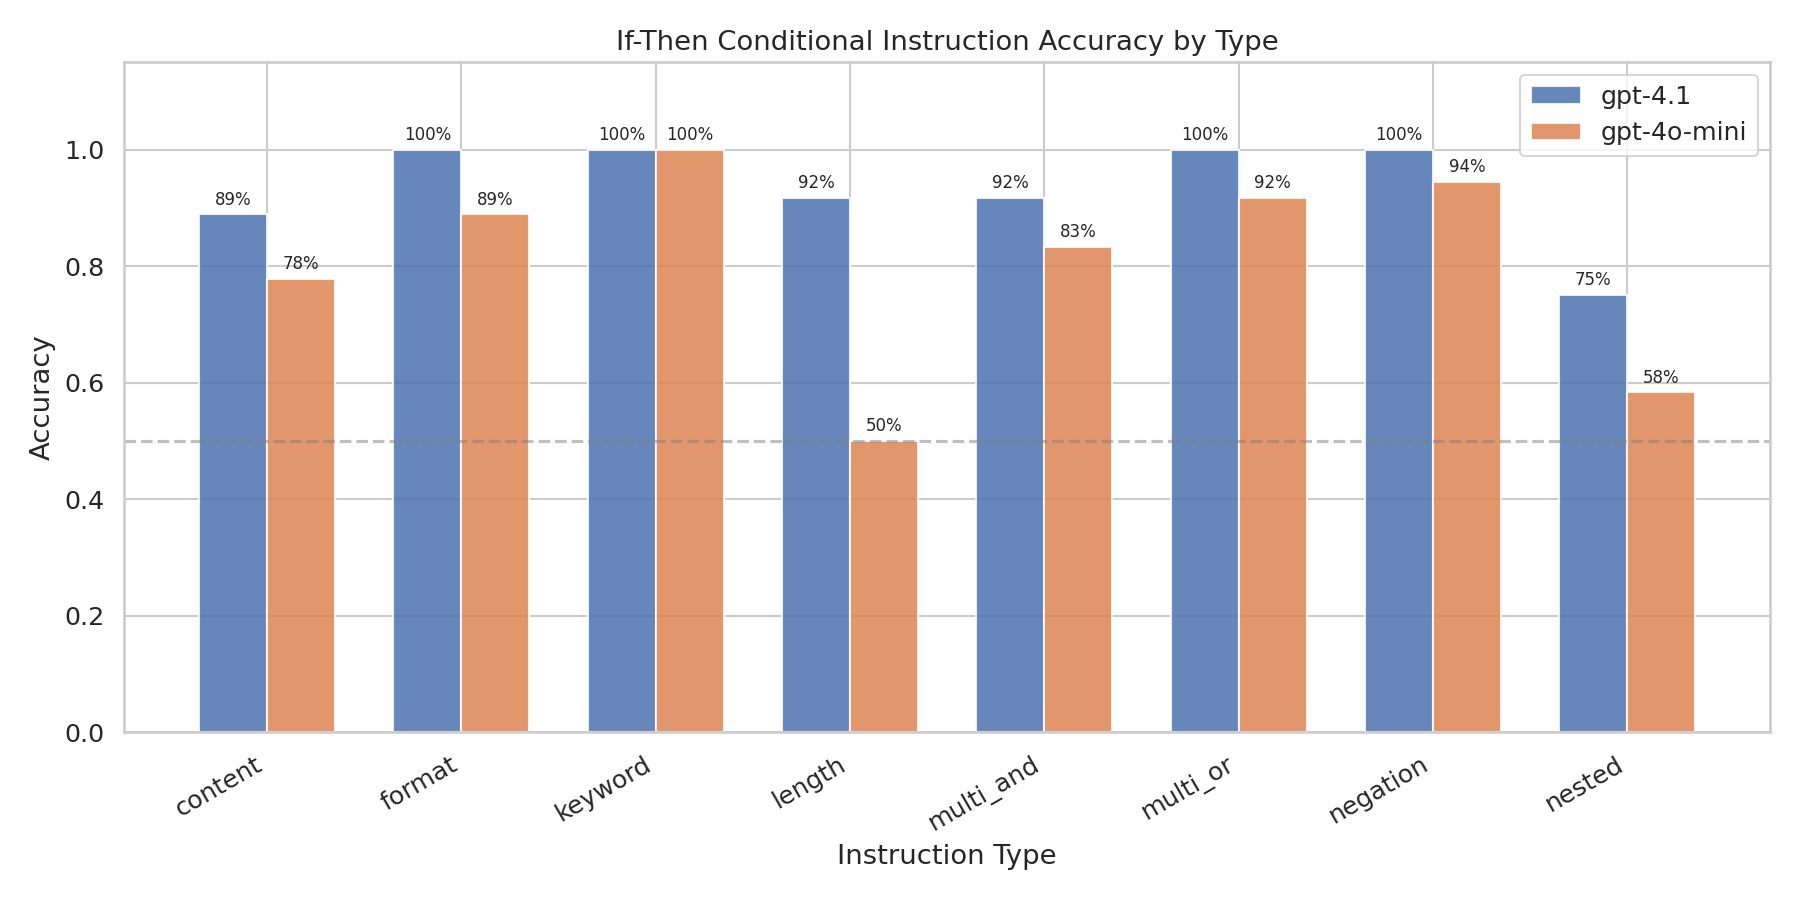
\includegraphics[width=0.95\linewidth]{figures/accuracy_by_type.png}
    \caption{Accuracy by conditional instruction type for both models. \gptlarge (dark) achieves perfect accuracy on 4 types but drops notably on \itype{Nested} and \itype{Content}. \gptsmall (light) shows a wider range, with \itype{Length} and \itype{Nested} being particularly challenging. The difficulty ordering is largely consistent across models.}
    \label{fig:accuracy}
\end{figure}

\subsection{Cross-Model Difficulty Consistency}

\Figref{fig:scatter} shows the per-type accuracy for \gptlarge versus \gptsmall. The Spearman rank correlation is $\rho = 0.83$ ($p = 0.011$), indicating a strong and statistically significant agreement in difficulty ranking. Both models find \itype{Keyword} easiest and \itype{Nested} hardest. This consistency suggests that the difficulty of conditional instruction types is an inherent property of the task rather than a model-specific weakness.

\begin{figure}[t]
    \centering
    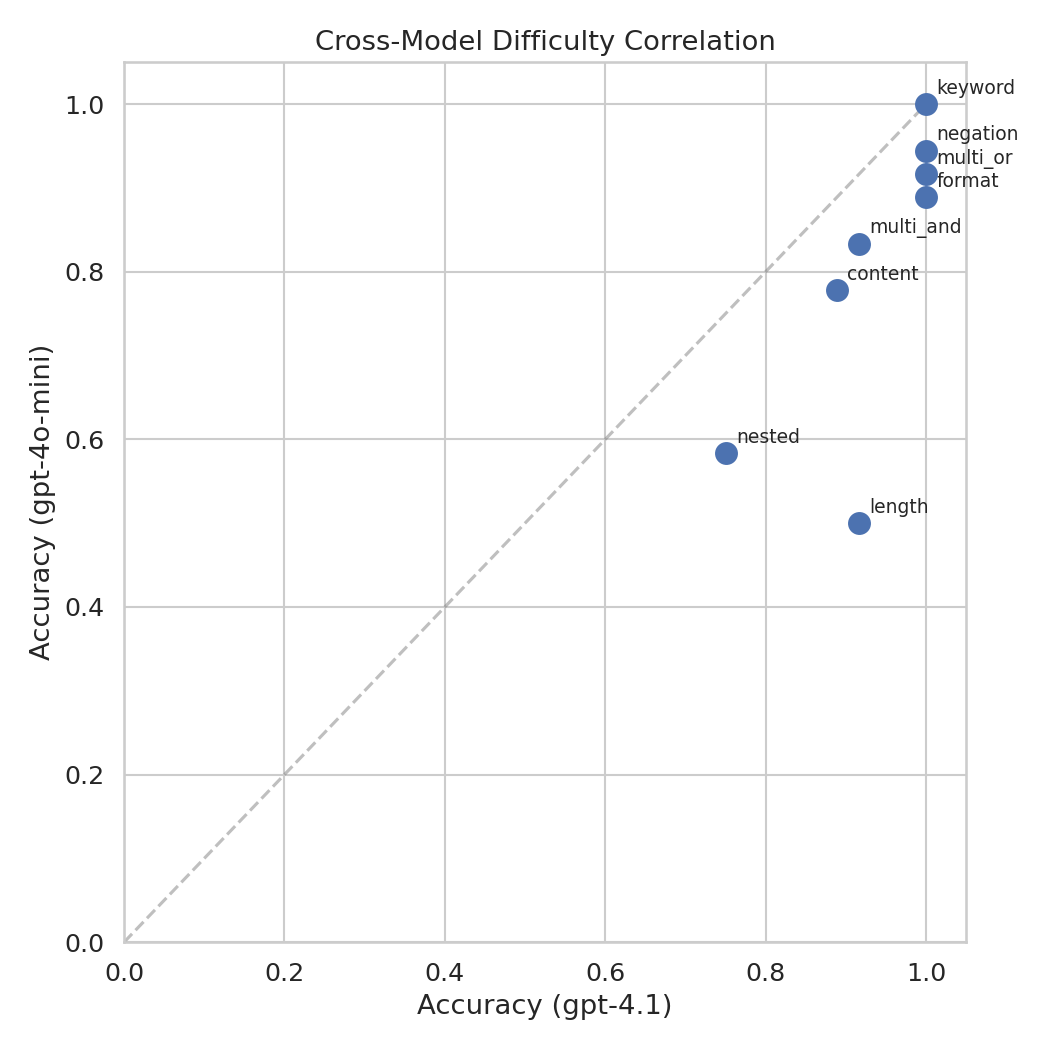
\includegraphics[width=0.65\linewidth]{figures/cross_model_scatter.png}
    \caption{Cross-model accuracy scatter plot. Each point is one instruction type. The strong positive correlation (Spearman $\rho = 0.83$, $p = 0.011$) indicates that the difficulty ranking of conditional instruction types is consistent across models.}
    \label{fig:scatter}
\end{figure}

\subsection{Error Analysis: False Positives vs.\ False Negatives}

\Tabref{tab:errors} breaks down errors into false positive rates (\FPR, over-triggering) and false negative rates (\FNR, under-triggering) for each model and instruction type. The two models exhibit strikingly different failure modes.

\para{\gptlarge predominantly over-triggers.}
\gptlarge's errors are concentrated in false positives: it performs the conditional action even when the condition is not met. The worst case is \itype{Nested} ($\FPR = 33.3\%$), followed by \itype{Content} ($\FPR = 22.2\%$) and \itype{Multi-AND} ($\FPR = 16.7\%$). The \itype{Content} false positives reveal semantic over-generalization---for example, when asked to include a hex color code only if a color is mentioned, the model included \texttt{\#228B22} (forest green) for an input about plants, associating the topic with the color green.

\para{\gptsmall predominantly under-triggers.}
\gptsmall's errors are concentrated in false negatives: it misses conditions that should fire. Most dramatically, \itype{Length} conditions have $\FNR = 100\%$---the model never correctly adjusts response length based on input properties. This is a consistent capability gap, not a stochastic failure. \itype{Nested} conditions also show high $\FNR$ ($33.3\%$) alongside high $\FPR$ ($50.0\%$), indicating general confusion rather than a directional bias.

\begin{table}[t]
    \centering
    \caption{False positive rate (\FPR) and false negative rate (\FNR) by instruction type. \gptlarge errors skew toward false positives (over-triggering), while \gptsmall errors skew toward false negatives (under-triggering). Highest error rates per model in \textbf{bold}.}
    \label{tab:errors}
    \resizebox{\textwidth}{!}{%
    \begin{tabular}{@{}lcccc@{}}
        \toprule
        & \multicolumn{2}{c}{\textbf{\gptlarge}} & \multicolumn{2}{c}{\textbf{\gptsmall}} \\
        \cmidrule(lr){2-3} \cmidrule(lr){4-5}
        \textbf{Type} & \FPR (\%) & \FNR (\%) & \FPR (\%) & \FNR (\%) \\
        \midrule
        \itype{Keyword}   & 0.0  & 0.0  & 0.0  & 0.0 \\
        \itype{Format}    & 0.0  & 0.0  & 11.1 & 11.1 \\
        \itype{Negation}  & 0.0  & 0.0  & 0.0  & 11.1 \\
        \itype{Multi-OR}  & 0.0  & 0.0  & 16.7 & 0.0 \\
        \itype{Multi-AND} & 16.7 & 0.0  & 16.7 & 16.7 \\
        \itype{Length}    & 0.0  & 16.7 & 0.0  & \textbf{100.0} \\
        \itype{Content}   & 22.2 & 0.0  & 22.2 & 22.2 \\
        \itype{Nested}   & \textbf{33.3} & 16.7 & \textbf{50.0} & 33.3 \\
        \bottomrule
    \end{tabular}
    }
\end{table}

\begin{figure}[t]
    \centering
    \begin{subfigure}[b]{0.48\textwidth}
        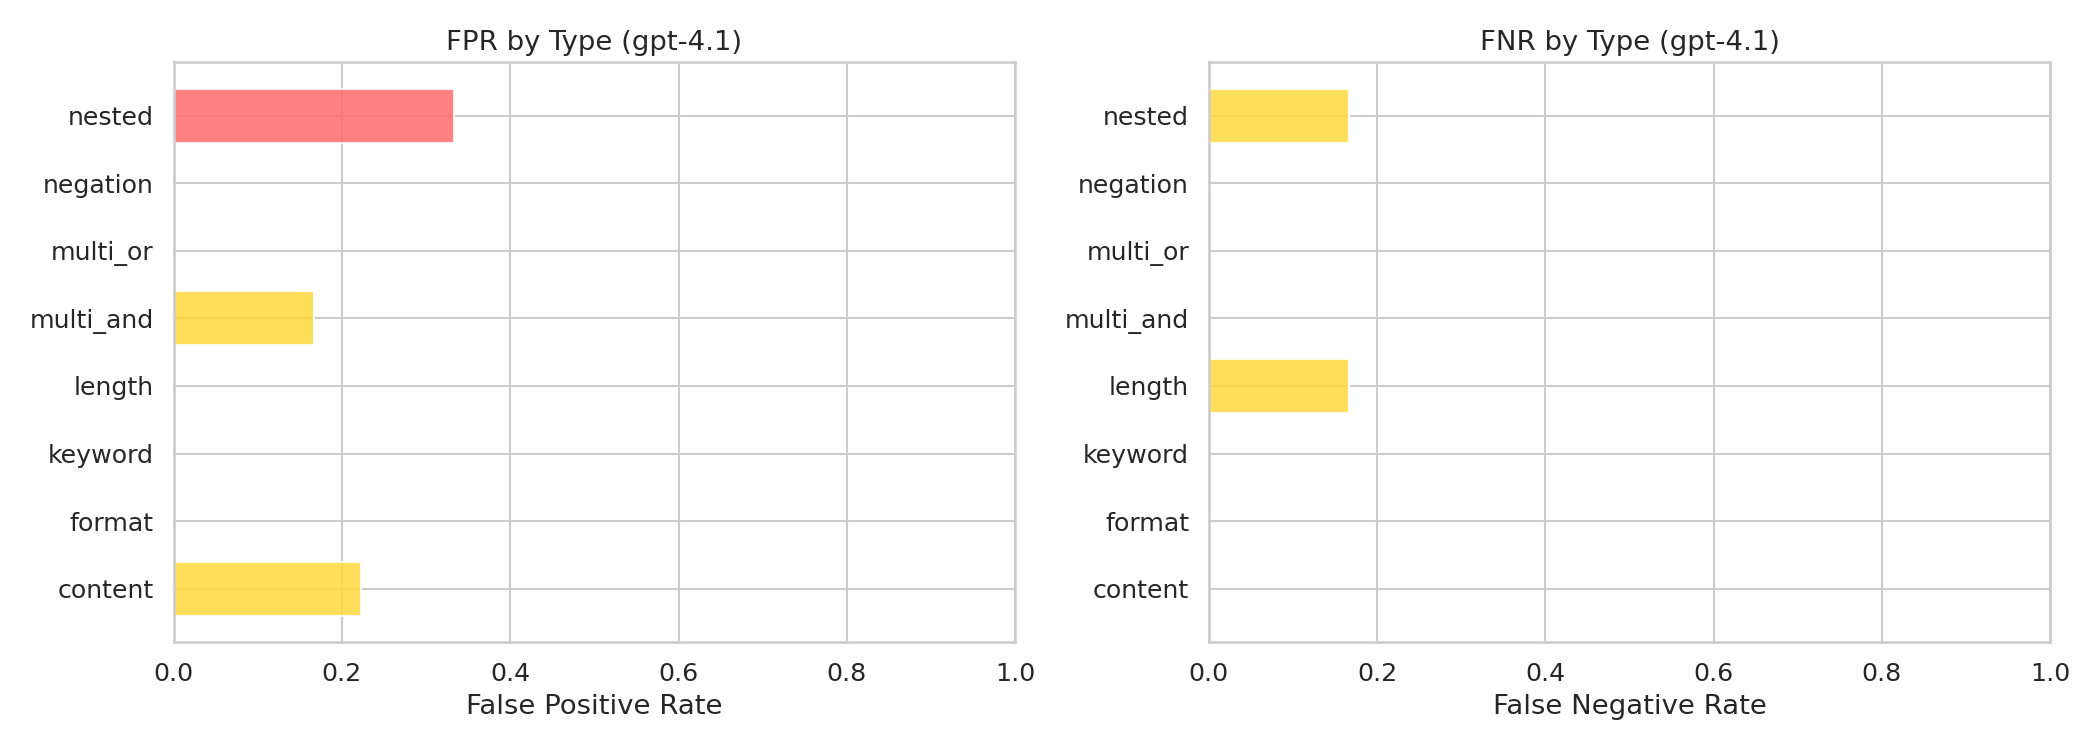
\includegraphics[width=\textwidth]{figures/fpr_fnr_gpt-4_1.png}
        \caption{\gptlarge}
        \label{fig:fpr_fnr_large}
    \end{subfigure}
    \hfill
    \begin{subfigure}[b]{0.48\textwidth}
        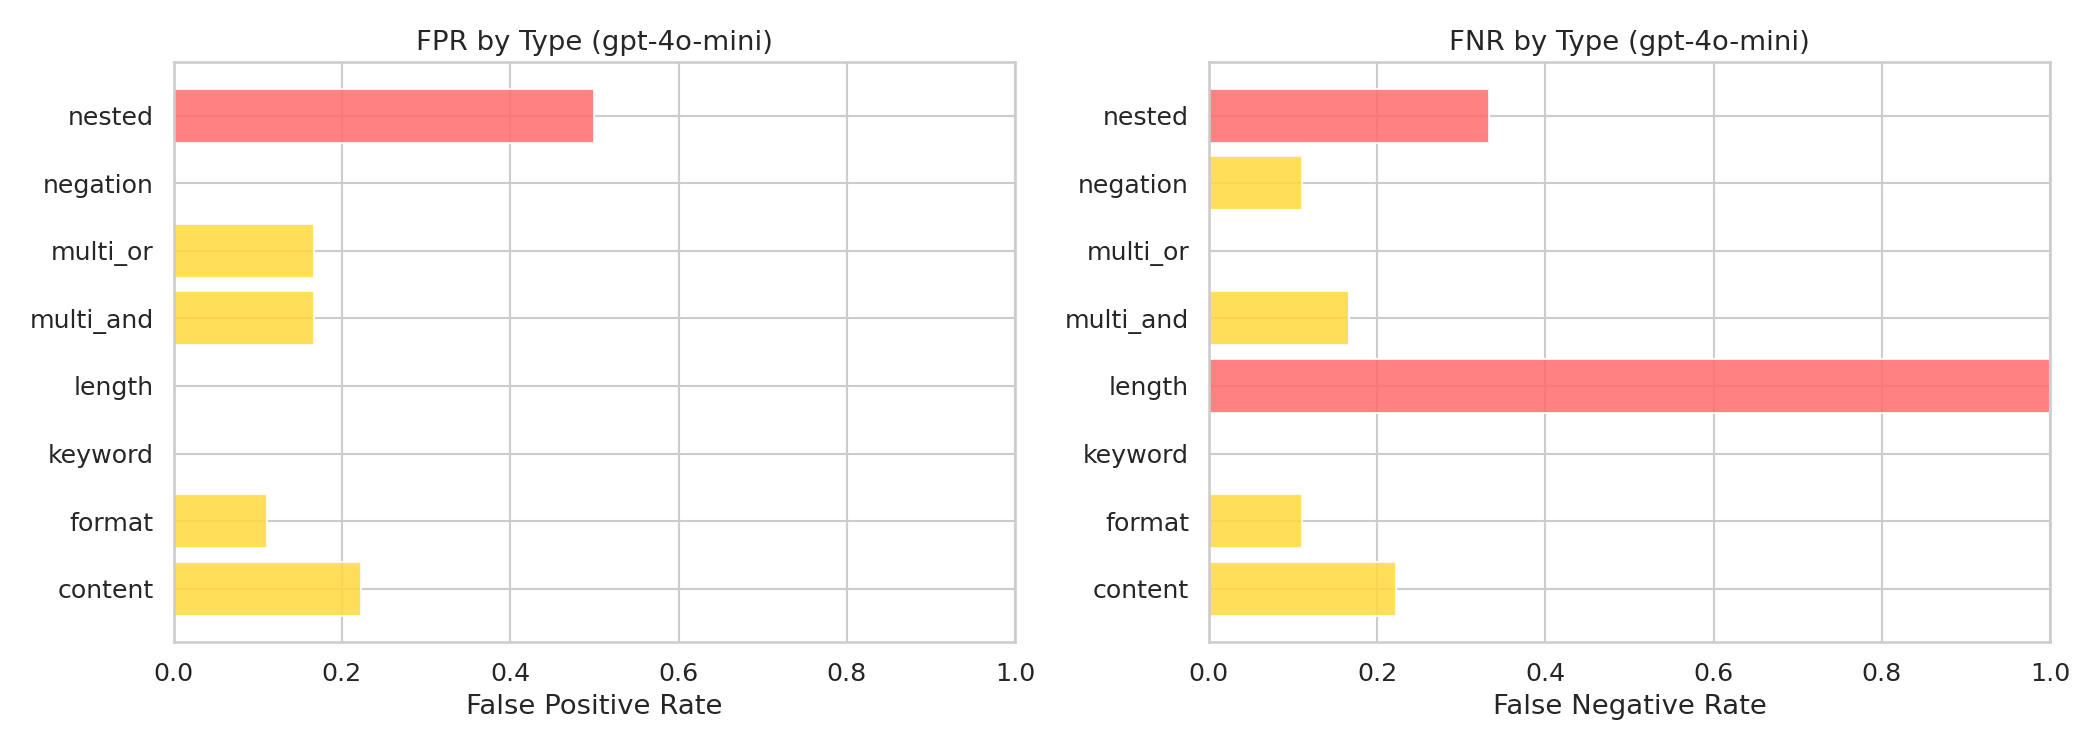
\includegraphics[width=\textwidth]{figures/fpr_fnr_gpt-4o-mini.png}
        \caption{\gptsmall}
        \label{fig:fpr_fnr_small}
    \end{subfigure}
    \caption{Error type breakdown by instruction type. \captiona~\gptlarge errors are dominated by false positives (over-triggering), especially for \itype{Nested} and \itype{Content}. \captionb~\gptsmall errors are dominated by false negatives (under-triggering), with \itype{Length} showing complete failure ($\FNR = 100\%$).}
    \label{fig:fpr_fnr}
\end{figure}

\subsection{Scaling with Multiple Conditions}
\label{sec:scaling_results}

\Tabref{tab:scaling} shows results from the scaling benchmark. Both models maintain near-perfect accuracy even with 4 simultaneous keyword-to-marker conditions. \gptlarge achieves 91.7\% overall accuracy with 2 conditions and recovers to 100\% with 4 conditions; \gptsmall achieves 100\% throughout. Per-marker accuracy (individual condition compliance within multi-condition prompts) remains $\geq$95.8\% for both models.

This result contrasts with the dramatic variation in the main benchmark. The key difference is that the scaling benchmark uses simple keyword-to-marker conditions---the easiest type. The capacity bottleneck is in the \emph{complexity} of individual conditions, not the \emph{number} of concurrent conditions (at least up to 4 simple conditions).

\begin{table}[t]
    \centering
    \caption{Scaling benchmark results. Overall accuracy requires all conditions in a prompt to be correct; per-marker accuracy measures individual condition compliance. Both models handle up to 4 simple concurrent conditions with minimal degradation.}
    \label{tab:scaling}
    \begin{tabular}{@{}lccc@{}}
        \toprule
        & \textbf{1 condition} & \textbf{2 conditions} & \textbf{4 conditions} \\
        \midrule
        \multicolumn{4}{@{}l}{\emph{Overall accuracy (\%)}} \\
        \quad \gptlarge & \textbf{100.0} & 91.7  & \textbf{100.0} \\
        \quad \gptsmall & \textbf{100.0} & \textbf{100.0} & \textbf{100.0} \\
        \midrule
        \multicolumn{4}{@{}l}{\emph{Per-marker accuracy (\%)}} \\
        \quad \gptlarge & --- & 95.8  & \textbf{100.0} \\
        \quad \gptsmall & --- & \textbf{100.0} & \textbf{100.0} \\
        \bottomrule
    \end{tabular}
\end{table}

\subsection{Difficulty Hierarchy}

Combining all results, we establish the following hierarchy of conditional instruction difficulty (averaged across both models, from easiest to hardest):

\begin{enumerate}[leftmargin=*,itemsep=0pt,topsep=0pt]
    \item \itype{Keyword} (100.0\%): Simple string-matching conditions are trivially reliable.
    \item \itype{Negation} (97.2\%): ``If NOT X'' conditions are handled surprisingly well.
    \item \itype{Multi-OR} (95.8\%): Disjunctive conditions are near-perfect.
    \item \itype{Format} (94.4\%): Format-switching on topic detection works well.
    \item \itype{Multi-AND} (87.5\%): Conjunctive conditions show some degradation.
    \item \itype{Content} (83.3\%): Semantic content detection is harder than keyword matching.
    \item \itype{Length} (70.8\%): Length control based on input properties is unreliable.
    \item \itype{Nested} (66.7\%): Multi-level conditional branching is the hardest.
\end{enumerate}
